\subsection*{Add.1}
\subsubsection*{(a)}
\paragraph{}
We could simplify the original fitting problem as follow:
\begin{align*}
&\min \sum_{i=1}^{m}((u_i-u_c)^2 +(v_i-v_c)^2-R^2)^2 \\
&\Rightarrow \min \sum_{i=1}^{m}(u_i^2 +v_i^2 - 2u_iu_c -2v_iv_c +(v_c^2 +u_c^2 -R^2))^2
\end{align*}
\paragraph{}
To write it into a linear least-square problem, we could have $a_i^T = [-2u_i -2v_i \ 1]^T$ and $b_i=-u_i^2 -v_i^2$, which are the row vectors of $A$ and $b$, and variable $x = [x_1\  x_2\  x_3]^T$.
\subsubsection*{(b)}
\paragraph{}
If we expand the normal equation with $A$ and $b$ we selected from (a), we get the following equation from the third row of expansion:
\begin{align*}
&2x_1\sum^n u_i+2x_2\sum^n v_i -nx_3= \sum^n(u_i^2+v_i^2) \\
&\Rightarrow nx_1^2+nx^2_2-nx_3=nx_1^2+nx^2_2-2x_1\sum^n u_i-2x_2\sum^n v_i+ \sum^n(u_i^2+v_i^2)\\
&\Rightarrow n(x_1^2+x^2_2-x_3) = \sum^n(x_1-u_i)^2 + \sum^n(x_2-v_i)^2 \geq 0
\end{align*}
\paragraph{}
i.e. $\hat{x}_1^2 +\hat{x}_2^2-\hat{x}_3 \geq 0$.
\subsubsection*{(c)}
Figure 1 presents the least-square fit of a circle to points.
\begin{figure}[h]
	\centering
	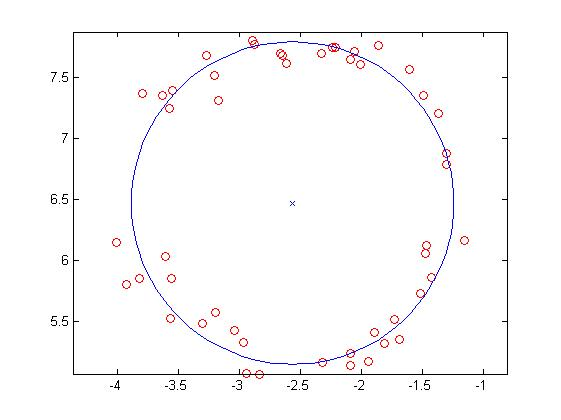
\includegraphics[scale=0.5]{fit}
	\caption{Least Square Fit}
\end{figure}